\documentclass[aspectratio=169,10pt]{beamer}

\usetheme{Madrid}
\usecolortheme{default}
\setbeamertemplate{navigation symbols}{}
\setbeamertemplate{footline}[frame number]

\usepackage{amsmath,amssymb,amsthm,booktabs,mathtools}
\usepackage{stmaryrd}
\usepackage{hyperref}
\usepackage{tikz}
\usetikzlibrary{arrows.meta,positioning,decorations.pathreplacing,calc,matrix}
\usepackage{pgfplots}
\pgfplotsset{compat=1.18}

% Semantic colors
\definecolor{positive}{HTML}{0173B2}
\definecolor{negative}{HTML}{DE8F05}
\definecolor{emphasis}{HTML}{029E73}
\definecolor{neutral}{gray}{0.55}
\definecolor{cbPurple}{HTML}{CC78BC}
\newcommand{\pos}[1]{\textcolor{positive}{#1}}
\renewcommand{\neg}[1]{\textcolor{negative}{#1}}
\newcommand{\HL}[1]{\textcolor{emphasis}{#1}}

% Domain macros
\newcommand{\F}{\mathbb{F}}
\newcommand{\N}{\mathbb{N}}
\newcommand{\Z}{\mathbb{Z}}
\newcommand{\tr}{\mathbf{tr}}
\newcommand{\WE}{\mathbf{W}_E}
\newcommand{\MLE}{\widetilde}
\newcommand{\eeq}{\widetilde{\mathrm{eq}}}

\title{zkAgent: Verifiable Agent Execution\\via One-Shot Complete LLM Inference Proof}
\author{Presenter: [name]}
\institute{Shanghai Jiao Tong University}
\date{}

\begin{document}

% ============================================================
% TITLE
% ============================================================
\begin{frame}
\titlepage
\vspace{-8pt}
{\small Joint work with [collaborators]}
\end{frame}

% ============================================================
% PART 1: OPENING & MOTIVATION
% ============================================================

\begin{frame}{Why Verifiable Agent Execution?}
LLM-based agents now manage \textbf{sensitive data} and \textbf{financial assets}:
\begin{itemize}
  \item Invoke business workflows, operate user-controlled resources, initiate payments
  \item Outsourced to third-party providers $\Rightarrow$ \neg{trust problem}
\end{itemize}

\vspace{6pt}
\begin{alertblock}{Threat: Malicious Provider}
\begin{enumerate}
  \item \neg{Model substitution} --- replace advertised model with cheaper/backdoored one
  \item \neg{Truncated generation} --- prematurely stop to reduce cost
  \item \neg{Tampered tool outputs} --- forge/censor web-search results or sandbox outputs
\end{enumerate}
\end{alertblock}

\vspace{4pt}
\textbf{Goal}: cryptographic proof that the published transcript is consistent with the \pos{committed model}, \pos{decoding rule}, and \pos{tool interfaces}.
\end{frame}

\begin{frame}{Three Challenges for Verifiable Agents}
\begin{columns}[T]
\column{0.48\textwidth}
\begin{exampleblock}{C1: Complete Inference}
Prior zkLLM proves only Transformer blocks.

Missing: \textbf{embedding lookup}, \textbf{positional encoding}, \textbf{decoding}.
\end{exampleblock}

\vspace{6pt}
\begin{exampleblock}{C2: Long Autoregressive Gen.}
Step-by-step proving: prover cost $\propto \sum_{i} i = O(T^2)$.

Need \textbf{batched} proof for entire transcript.
\end{exampleblock}

\column{0.48\textwidth}
\begin{exampleblock}{C3: Tool Interactions}
Agent interleaves LLM tokens with \textbf{externally injected} tool observations.

Must bind tool outputs cryptographically.
\end{exampleblock}

\vspace{6pt}
\begin{block}{Our Answer: zkAgent}
\begin{itemize}
  \item \pos{Complete} inference proof (C1)
  \item \pos{One-shot} transcript proving (C2)
  \item \pos{Verifiable} tool binding (C3)
\end{itemize}
\end{block}
\end{columns}
\end{frame}

% ============================================================
% PART 2: BRIEF BACKGROUND
% ============================================================

\begin{frame}{Background: LLM Inference Pipeline}
\begin{center}
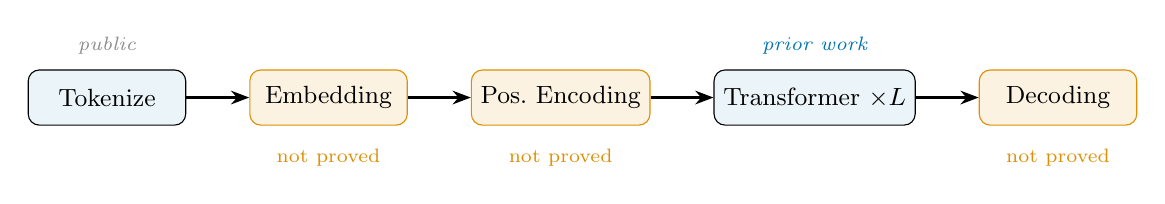
\begin{tikzpicture}[
  box/.style={draw, rounded corners, minimum width=2.0cm, minimum height=0.7cm,
              font=\small, fill=positive!8},
  omit/.style={draw, rounded corners, minimum width=2.0cm, minimum height=0.7cm,
               font=\small, fill=negative!12, draw=negative},
  arr/.style={-{Stealth}, thick},
  scale=0.95
]
  \node[box] (tok) {Tokenize};
  \node[omit, right=0.8cm of tok] (emb) {Embedding};
  \node[omit, right=0.8cm of emb] (pos) {Pos.\ Encoding};
  \node[box, right=0.8cm of pos] (tfm) {Transformer $\times L$};
  \node[omit, right=0.8cm of tfm] (dec) {Decoding};

  \draw[arr] (tok) -- (emb);
  \draw[arr] (emb) -- (pos);
  \draw[arr] (pos) -- (tfm);
  \draw[arr] (tfm) -- (dec);

  \node[above=2pt of tok, font=\scriptsize\itshape, text=neutral] {public};
  \node[below=5pt of emb, font=\scriptsize, text=negative] {not proved};
  \node[below=5pt of pos, font=\scriptsize, text=negative] {not proved};
  \node[above=2pt of tfm, font=\scriptsize\itshape, text=positive] {prior work};
  \node[below=5pt of dec, font=\scriptsize, text=negative] {not proved};
\end{tikzpicture}
\end{center}

\vspace{4pt}
Key components (for crypto audience):
\begin{itemize}
  \item \textbf{Embedding}: token id $t_i \in [N]$ $\mapsto$ row $\WE[t_i,:] \in \F^d$ \quad ($N \approx 50\text{K}$, $d = 768$ for GPT-2)
  \item \textbf{Positional encoding}: inject position info (APE: additive; \textbf{RoPE}: per-head rotation)
  \item \textbf{Transformer}: $L$ layers of self-attention + FFN, proved by GKR + lookup
  \item \textbf{Decoding}: logits $\boldsymbol{\ell} \in \F^N \to$ next token via argmax / top-$k$ / top-$p$
\end{itemize}
\end{frame}

\begin{frame}{Background: Agent = LLM + Tools}
\begin{center}
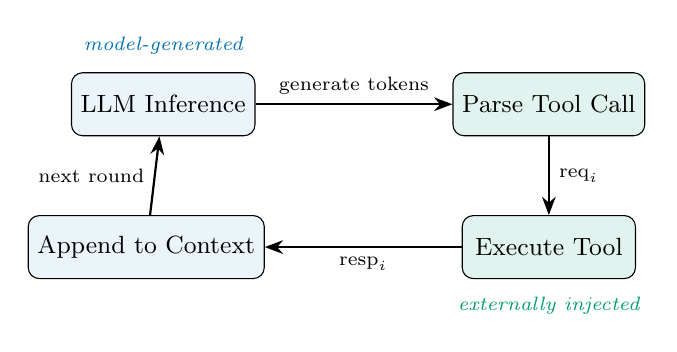
\begin{tikzpicture}[
  box/.style={draw, rounded corners, minimum width=2.2cm, minimum height=0.8cm,
              font=\small, fill=positive!8},
  tool/.style={draw, rounded corners, minimum width=2.2cm, minimum height=0.8cm,
               font=\small, fill=emphasis!12},
  arr/.style={-{Stealth}, thick},
]
  \node[box] (llm) {LLM Inference};
  \node[tool, right=2.5cm of llm] (parse) {Parse Tool Call};
  \node[tool, below=1.0cm of parse] (exec) {Execute Tool};
  \node[box, left=2.5cm of exec] (append) {Append to Context};

  \draw[arr] (llm) -- node[above, font=\scriptsize] {generate tokens} (parse);
  \draw[arr] (parse) -- node[right, font=\scriptsize] {$\mathrm{req}_i$} (exec);
  \draw[arr] (exec) -- node[below, font=\scriptsize] {$\mathrm{resp}_i$} (append);
  \draw[arr] (append) -- node[left, font=\scriptsize] {next round} (llm);

  \node[above=3pt of llm, font=\scriptsize\itshape, text=positive] {model-generated};
  \node[below=3pt of exec, font=\scriptsize\itshape, text=emphasis] {externally injected};
\end{tikzpicture}
\end{center}

\vspace{4pt}
\textbf{Transcript} $\tr = (t_0, \ldots, t_{T-1}) \in [N]^T$: chronological sequence of all tokens.

Segments: user messages $\mid$ LLM outputs $\mid$ tool-call spans $\mid$ tool-observation spans.

\vspace{4pt}
Proving challenge: transcript interleaves \pos{model-generated} and \HL{externally injected} tokens. Must verify \emph{both}.
\end{frame}

\begin{frame}{ZK Building Blocks (Quick Review)}
\begin{columns}[T]
\column{0.48\textwidth}
\textbf{GKR Protocol}
\begin{itemize}
  \item Interactive proof for layered arithmetic circuits
  \item Prover reduces claim layer-by-layer via \textbf{sumcheck}
  \item Avoids committing to full execution trace
  \item ML-friendly variant: gates can read from input layer directly
\end{itemize}

\vspace{6pt}
\textbf{Sumcheck Protocol}
\begin{itemize}
  \item Proves $v = \sum_{\mathbf{x} \in \{0,1\}^n} f(\mathbf{x})$
  \item Core building block of GKR
\end{itemize}

\column{0.48\textwidth}
\textbf{Lookup Arguments}
\begin{itemize}
  \item Prove multiset inclusion $\{a_i\} \subseteq \{b_j\}$
  \item Used for non-linear ops (exp, ReLU) and range checks
\end{itemize}

\vspace{4pt}
Three regimes in practice:
\begin{enumerate}
  \item \textbf{Small tables} ($8$--$16$ bit): cost $\sim \ell + N$
  \item \textbf{Large structured}: decompose into smaller parts
  \item \textbf{Huge unstructured} (embedding): need \textbf{preprocessing} to decouple online cost from $N$
\end{enumerate}

\vspace{4pt}
We use: \textbf{Shout} (small tables), \textbf{cq} (preprocessed lookup for embedding).
\end{columns}
\end{frame}

% ============================================================
% PART 3: COMPLETE INFERENCE PROOF
% ============================================================

\begin{frame}{Complete Inference: What Was Missing?}
\begin{center}
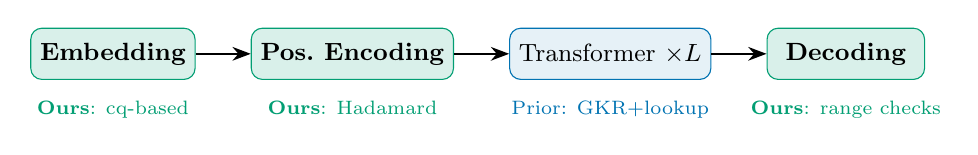
\begin{tikzpicture}[
  proved/.style={draw, rounded corners, minimum width=2.0cm, minimum height=0.65cm,
                 font=\small, fill=positive!10, draw=positive},
  new/.style={draw, rounded corners, minimum width=2.0cm, minimum height=0.65cm,
              font=\small\bfseries, fill=emphasis!15, draw=emphasis},
  arr/.style={-{Stealth}, thick},
]
  \node[new] (emb) {Embedding};
  \node[new, right=0.7cm of emb] (pos) {Pos.\ Encoding};
  \node[proved, right=0.7cm of pos] (tfm) {Transformer $\times L$};
  \node[new, right=0.7cm of tfm] (dec) {Decoding};

  \draw[arr] (emb) -- (pos);
  \draw[arr] (pos) -- (tfm);
  \draw[arr] (tfm) -- (dec);

  \node[below=4pt of emb, font=\scriptsize, text=emphasis] {\textbf{Ours}: cq-based};
  \node[below=4pt of pos, font=\scriptsize, text=emphasis] {\textbf{Ours}: Hadamard};
  \node[below=4pt of tfm, font=\scriptsize, text=positive] {Prior: GKR+lookup};
  \node[below=4pt of dec, font=\scriptsize, text=emphasis] {\textbf{Ours}: range checks};
\end{tikzpicture}
\end{center}

\vspace{6pt}
\begin{tabular}{@{}llll@{}}
\toprule
Component & Challenge & Our approach & Cost \\
\midrule
Embedding & Table size $Nd \approx 2^{25}$ & Preprocessed cq lookup & $O(Td)$ online \\
RoPE & Naïve: $O(Td_h^2)$ matmul & Hadamard + permutation & $O(Td_h)$ \\
Decoding & Non-arithmetic comparisons & Signed range checks (Shout) & $O(N)$ per step \\
\bottomrule
\end{tabular}
\end{frame}

\begin{frame}{Token-to-Embedding Lookup: Idea}
\textbf{Goal}: prove $\mathbf{H}_0[i,:] = \WE[t_i,:]$ for all $i \in [T]$.

\vspace{4pt}
Naïve approach: $d$ independent column lookups into size-$N$ table $\Rightarrow$ \neg{vulnerable to mix-and-match attack} (splice coordinates from different rows).

\vspace{6pt}
\begin{alertblock}{Key Idea: Row Binding via Random Folding}
Sample challenge $\rho$ after committing to $\mathbf{H}_0$. Define folded scalars:
\[
  b_u := u + \sum_{j \in [d]} \rho^{j+1} \cdot \WE[u,j], \qquad
  a_i := t_i + \sum_{j \in [d]} \rho^{j+1} \cdot \mathbf{H}_0[i,j].
\]
\end{alertblock}

Reduce to \textbf{multiset inclusion}: $\{a_i\}_{i \in [T]} \subseteq \{b_u\}_{u \in [N]}$.

\vspace{4pt}
\textbf{Soundness}: if $\mathbf{H}_0[i,:] \neq \WE[t_i,:]$, then $a_i = b_{t_i}$ requires degree-$d$ polynomial to vanish at $\rho$ $\Rightarrow$ probability $\leq d/|\F|$.
\end{frame}

\begin{frame}{Token-to-Embedding Lookup: Protocol}
\begin{columns}[T]
\column{0.48\textwidth}
\textbf{One-time preprocessing} (per model):

Preprocess each column of $\WE$ independently:
\[
  \mathrm{pp}_{\mathrm{idx}} \gets \mathrm{Preproc}(\mathrm{idx}), \quad
  \mathrm{pp}_{E,j} \gets \mathrm{Preproc}(\mathbf{w}_j)
\]
After sampling $\rho$ online, fold:
\[
  \mathrm{pp}_\rho := \mathrm{pp}_{\mathrm{idx}} + \sum_{j \in [d]} \rho^{j+1}\, \mathrm{pp}_{E,j}
\]
\pos{KZG linearity} enables this without re-preprocessing.

\column{0.48\textwidth}
\textbf{Online proving}:

\textit{Table side}: logarithmic-derivative witnesses
\[
  f_u = \frac{m_u}{b_u + \beta}, \quad z = \sum_{u \in [N]} f_u
\]
Divisibility check via cq pairing. Cost: $O(T)$ (sparse support).

\vspace{4pt}
\textit{Query side}: multilinear extension world
\[
  \MLE{a}_\rho(\mathbf{x}) = \MLE{t}(\mathbf{x}) + \MLE{s}_\rho(\mathbf{x})
\]
Batched sumcheck verifies $z = \sum_{i} 1/(a_i + \beta)$.

Reuses commitment to $\mathbf{H}_0$ from downstream GKR.
\end{columns}

\vspace{6pt}
\pos{Online prover}: $O(Td)$ field + group ops. \quad \pos{Verifier}: $O(\log T + \log d)$.
\end{frame}

\begin{frame}{Efficient Proof for RoPE}
\textbf{RoPE} applies position-dependent 2$\times$2 rotations to Query/Key vectors.

Naïve arithmetization [zkLLM]: treat as matrix-vector multiplications $\Rightarrow$ $O(Td_h^2)$.

\vspace{6pt}
\begin{exampleblock}{Our Approach: Hadamard + Permutation}
Define permutation $\pi(\mathbf{u}) = (-u_1, u_0, -u_3, u_2, \ldots)$ and precomputed $\mathbf{c}_m, \mathbf{s}_m \in \F^{d_h}$:
\[
  \mathbf{Q}^{\mathrm{rot}} = \mathbf{Q} \circ \mathbf{C} + \pi(\mathbf{Q}) \circ \mathbf{S}, \qquad
  \mathbf{K}^{\mathrm{rot}} = \mathbf{K} \circ \mathbf{C} + \pi(\mathbf{K}) \circ \mathbf{S}
\]
\end{exampleblock}

\vspace{4pt}
\begin{itemize}
  \item $\pi(\cdot)$: fixed wiring (free in GKR circuit)
  \item $\mathbf{C}, \mathbf{S}$: public constants (precomputed from position frequencies)
  \item Only \textbf{two Hadamard products} per tensor $\Rightarrow$ $O(Td_h)$ per head
\end{itemize}

\vspace{4pt}
\textbf{Practical impact}: Llama-2-7B RoPE proving: $95.70$s $\to$ $3.06$s per layer, saving \pos{2,964s} across 32 layers.
\end{frame}

\begin{frame}{Decoding Procedure}
Map final logits $\boldsymbol{\ell} = (\ell_0, \ldots, \ell_{N-1}) \in \F^N$ to output token $y \in [N]$.

\vspace{4pt}
\begin{columns}[T]
\column{0.48\textwidth}
\textbf{Greedy decoding} ($y = \mathrm{argmax}\;\ell_i$):

Prover supplies differences $\Delta_i := \ell_y - \ell_i$.

Constraints:
\begin{itemize}
  \item $\Delta_y = 0$
  \item $\Delta_i \in [0, 2B)$ for all $i \in [N]$
\end{itemize}

Enforced via \textbf{signed range checks} (Shout).

\column{0.48\textwidth}
\textbf{Top-$k$ decoding}:

Prover supplies candidate set $S$ ($|S| = k$), selector $\boldsymbol{\chi} \in \{0,1\}^N$, threshold $\lambda$:
\begin{itemize}
  \item $\chi_i(\ell_i - \lambda) \in [0, 2B)$ \quad (selected: $\ell_i \geq \lambda$)
  \item $(1-\chi_i)(\lambda - \ell_i) \in [0, 2B)$ \quad (rejected: $\ell_i \leq \lambda$)
  \item Softmax only over $S$ $\Rightarrow$ cost $O(T|S|)$
\end{itemize}
\end{columns}

\vspace{8pt}
\textbf{Softmax}: multiplicative form $p_i \cdot D = \theta \cdot e_i$, exponentiation via digit decomposition + lookup tables (following zkGPT).

\vspace{2pt}
\textbf{Cost}: $O(N)$ range checks for greedy; top-$k$ adds $O(T|S|)$ for Softmax; top-$p$ adds $O(TN)$.
\end{frame}

\begin{frame}{Complete Inference: Summary}
\begin{center}
\begin{tabular}{@{}lccl@{}}
\toprule
\textbf{Component} & \textbf{Online Prover} & \textbf{Verifier} & \textbf{Key technique} \\
\midrule
Embedding lookup & $O(Td)$ & $O(\log T + \log d)$ & Preprocessed cq \\
RoPE & $O(Td_h)$ & native GKR & Hadamard form \\
APE & $O(Td)$ & native GKR & Linear addition \\
Transformer $\times L$ & (prior work) & (prior work) & GKR + Shout \\
Greedy decoding & $O(N)$ per step & $O(\log N)$ & Signed range checks \\
Top-$k$ Softmax & $O(T|S|)$ & $O(\log |S|)$ & Digit decomp.\ + lookup \\
\bottomrule
\end{tabular}
\end{center}

\vspace{6pt}
\textbf{Embedding preprocessing}: one-time $O(dN\log N)$, amortized across all future inferences.

\vspace{4pt}
Result: first system proving the \pos{complete pipeline} from discrete tokens to output token.
\end{frame}

% ============================================================
% PART 4: ONE-SHOT TRANSCRIPT PROVING
% ============================================================

\begin{frame}{Step-by-Step Proving is Too Expensive}
Standard autoregressive generation: token $t_{i+1}$ depends on prefix $\tr_{\leq i}$.

\vspace{4pt}
\textbf{Step-by-step approach}: prove each step separately.
\begin{itemize}
  \item Step $i$: forward pass on context length $i$ $\Rightarrow$ prover cost $\propto i$
  \item Total: $\sum_{i=T_0}^{T-1} i = O(T^2)$ \quad \neg{quadratic!}
\end{itemize}

\vspace{4pt}
\begin{alertblock}{Concrete Numbers (GPT-2, $T_0=30$, $T=512$)}
\begin{tabular}{@{}lrr@{}}
\toprule
& \textbf{zkGPT (step-by-step)} & \textbf{zkAgent (one-shot)} \\
\midrule
Prove time & 149,192.6\,s ($\approx$ 41.4 hours) & \pos{508.46\,s} \\
Verify time & 4,361.09\,s & \pos{0.51\,s} \\
Per token & 309\,s/token & \pos{1.05\,s/token} \\
\bottomrule
\end{tabular}
\end{alertblock}

\pos{294$\times$} prover speedup, \pos{9,690$\times$} verifier speedup.
\end{frame}

\begin{frame}{Key Insight: Causal Attention Mask}
\label{slide:masking}
The prover already knows the \textbf{full transcript} $\tr$.

\textbf{Idea}: run one teacher-forced forward pass on entire $\tr$, get all logits in parallel.

\vspace{4pt}
\textbf{Problem}: naïve full-sequence evaluation lets position $i$ attend to future tokens $t_{>i}$.

\vspace{4pt}
\begin{exampleblock}{Solution: Causal Mask in Self-Attention}
\[
  \mathrm{Attn}(\mathbf{Q}, \mathbf{K}, \mathbf{V}) = \mathrm{softmax}\!\left(\frac{\mathbf{Q}\mathbf{K}^\top + \mathbf{M}^{\mathrm{cau}}}{\sqrt{d_h}}\right)\mathbf{V}
\]
where $M^{\mathrm{cau}}_{ij} = 0$ if $j \leq i$, $\;-\infty$ otherwise.
\end{exampleblock}

\vspace{4pt}
\textbf{Prefix equivalence} (Appendix D): under causal mask, logits at position $i$ depend \emph{only} on $\tr_{\leq i}$, identical to running LLM on the prefix alone.

$\Rightarrow$ One forward pass + per-position decoding check = full autoregressive proof.
\end{frame}

\begin{frame}{One-Shot Proving: Formal Construction}
\begin{columns}[T]
\column{0.45\textwidth}
\begin{center}
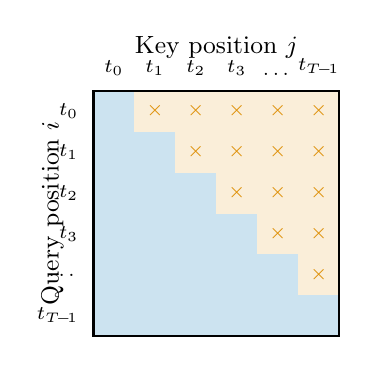
\begin{tikzpicture}[scale=0.52, every node/.style={font=\small}]
  \def\sz{6}
  \foreach \i in {0,...,5} {
    \foreach \j in {0,...,5} {
      \pgfmathparse{int(\j <= \i)}
      \ifnum\pgfmathresult=1
        \fill[positive!20] (\j, \sz-1-\i) rectangle (\j+1, \sz-\i);
      \else
        \fill[negative!15] (\j, \sz-1-\i) rectangle (\j+1, \sz-\i);
        \node[font=\scriptsize, text=negative] at (\j+0.5, \sz-0.5-\i) {$\times$};
      \fi
    }
  }
  \draw[thick] (0,0) rectangle (\sz, \sz);
  \node[above=8pt, font=\small] at (3, \sz) {Key position $j$};
  \node[rotate=90, font=\small] at (-1.0, 3) {Query position $i$};
  \foreach \i/\tok in {0/$t_0$, 1/$t_1$, 2/$t_2$, 3/$t_3$, 4/\ldots, 5/$t_{T\!-\!1}$} {
    \node[font=\scriptsize, above=2pt] at (\i+0.5, \sz) {\tok};
    \node[font=\scriptsize, left=2pt] at (0, \sz-0.5-\i) {\tok};
  }
\end{tikzpicture}
\end{center}

\vspace{2pt}
{\small \pos{Blue}: attend ($j \leq i$) \quad \neg{Orange}: masked ($j > i$)}

\column{0.52\textwidth}
\textbf{Shift constraint}:

$\forall\, i \in \{T_0\!-\!1, \ldots, T\!-\!2\}$:
\[
  g_i = 1 \;\Rightarrow\; t_{i+1} = \mathrm{Dec}(\boldsymbol{\ell}_i)
\]

Causal mask guarantees logits at position $i$ depend only on $\tr_{\leq i}$.

One forward pass $+$ per-position check $=$ full autoregressive proof.
\end{columns}

\vspace{2pt}
\textbf{Circuit}: materialize scores $\{s_{ij}\}_{j \leq i}$ only $\Rightarrow$ exponentiation lookups: $T^2 \to T(T+1)/2$.
\end{frame}

\begin{frame}{From Single Continuation to Agent Traces}
Agent transcripts interleave model-generated and externally injected tokens.

\vspace{4pt}
\textbf{Generation mask} $\mathbf{g} = (g_0, \ldots, g_{T-2}) \in \{0,1\}^{T-1}$:
\[
  g_i = \begin{cases}
    1 & t_{i+1} \text{ is produced by } \mathrm{LLM}_W \text{ from prefix } \tr_{\leq i} \\
    0 & t_{i+1} \text{ is externally injected (tool observation)}
  \end{cases}
\]

Enforce decoding only on model-generated transitions:
\[
  \forall\, i: \quad g_i = 1 \;\Rightarrow\; t_{i+1} = \mathrm{Dec}(\boldsymbol{\ell}_i)
\]

\vspace{4pt}
\begin{columns}[T]
\column{0.48\textwidth}
\textbf{Security of $\mathbf{g}$}:
\begin{itemize}
  \item $\mathbf{g}$ derived from public transcript grammar, \textbf{not chosen by prover}
  \item Hidden reasoning: provider publishes commitment $c_R$ and length $L_R$
  \item Early termination: grammar requires EOS at end of each model span
\end{itemize}

\column{0.48\textwidth}
\textbf{Multi-inference in one proof}:
\begin{itemize}
  \item Multiple LLM invocations in agent loop
  \item All handled by \textbf{single} masked forward pass
  \item $g_i = 0$ at tool-observation positions $\Rightarrow$ no decoding constraint
\end{itemize}
\end{columns}
\end{frame}

% ============================================================
% PART 5: VERIFIABLE TOOL BINDING
% ============================================================

\begin{frame}{Verifiable Tool Binding: Overview}
\begin{center}
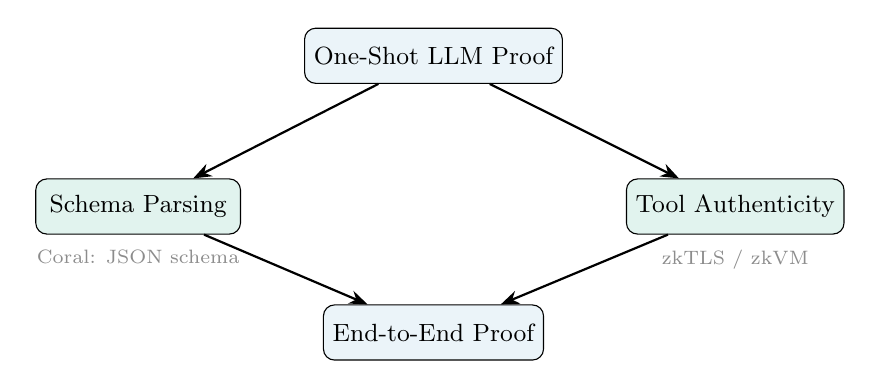
\begin{tikzpicture}[
  box/.style={draw, rounded corners, minimum width=2.6cm, minimum height=0.7cm,
              font=\small, fill=positive!8},
  tbox/.style={draw, rounded corners, minimum width=2.6cm, minimum height=0.7cm,
               font=\small, fill=emphasis!12},
  arr/.style={-{Stealth}, thick},
]
  \node[box] (transcript) {One-Shot LLM Proof};
  \node[tbox, below left=1.2cm and 0.8cm of transcript] (schema) {Schema Parsing};
  \node[tbox, below right=1.2cm and 0.8cm of transcript] (tool) {Tool Authenticity};
  \node[box, below=2.8cm of transcript] (compose) {End-to-End Proof};

  \draw[arr] (transcript) -- (schema);
  \draw[arr] (transcript) -- (tool);
  \draw[arr] (schema) -- (compose);
  \draw[arr] (tool) -- (compose);

  \node[below=2pt of schema, font=\scriptsize, text=neutral] {Coral: JSON schema};
  \node[below=2pt of tool, font=\scriptsize, text=neutral] {zkTLS / zkVM};
\end{tikzpicture}
\end{center}

\vspace{4pt}
\textbf{Three guarantees composed}:
\begin{enumerate}
  \item \textbf{Model integrity}: all model-generated tokens satisfy decoding constraint
  \item \textbf{Tool-call integrity}: each tool-call span is well-formed JSON per public schema (Coral)
  \item \textbf{Tool integrity}: each tool observation is authentic output of the claimed tool
\end{enumerate}
\end{frame}

\begin{frame}{Tool Binding: APIs and Code Execution}
\begin{columns}[T]
\column{0.48\textwidth}
\textbf{Remote APIs via zkTLS}

For invocation $i$ with server $\mathrm{id}_i$:
\[
  \mathrm{Verify}_{\mathrm{io}}(\mathrm{id}_i, \mathrm{req}_i, \mathrm{resp}_i, \pi^{\mathrm{io}}_i) = 1
\]
\begin{itemize}
  \item Cryptographically binds response to request under server identity
  \item Proves \textbf{provenance}, not correctness of external service
  \item Binding: $\mathrm{resp}_i$ embedded into $\tr$ as exact token span
\end{itemize}

\column{0.48\textwidth}
\textbf{Local Code via zkVM}

Pipeline: Python $\xrightarrow{\text{Depyler}}$ Rust $\xrightarrow{\text{compile}}$ RISC-V $\xrightarrow{\text{SP1}}$ proof
\[
  \mathrm{Verify}_{\mathrm{vm}}(\mathrm{Rust}(\mathrm{prog}_i), \mathrm{output}_i, \pi^{\mathrm{vm}}_i) = 1
\]
\begin{itemize}
  \item Deterministic execution semantics
  \item $\mathrm{prog}_i$ and $\mathrm{Rust}(\mathrm{prog}_i)$ public for independent verification
  \item Output bound to transcript span
\end{itemize}
\end{columns}

\vspace{8pt}
\textbf{Composition}: tool subproofs composed with one-shot transcript proof $\Rightarrow$ \pos{single end-to-end statement}.
\end{frame}

% ============================================================
% PART 6: EVALUATION
% ============================================================

\begin{frame}{Evaluation: Embedding Lookup Benchmark}
\textbf{GPT-2 embedding table}: $N = 50{,}257$, $d = 768$, 32 threads.

\vspace{4pt}
\begin{columns}[T]
\column{0.48\textwidth}
\textbf{One-time preprocessing}:

\vspace{2pt}
\begin{tabular}{@{}lrr@{}}
\toprule
Method & Time (s) & Size (GB) \\
\midrule
Segment Lkup & 8,747.7 & 6.50 \\
Campanelli et al. & 11,296.9 & 48.00 \\
\textbf{Ours} & \pos{\textbf{759.9}} & \pos{\textbf{4.52}} \\
\bottomrule
\end{tabular}

\pos{11.5$\times$} faster preprocessing.

\column{0.48\textwidth}
\textbf{Online proving} (selected $T$):

\vspace{2pt}
\begin{tabular}{@{}lrrr@{}}
\toprule
$T$ & Ours & Seg.\ Lkup & LogUp \\
\midrule
$2^5$ & \pos{0.035s} & 4.98s & 123.6s \\
$2^8$ & \pos{0.10s} & 9.75s & 136.0s \\
$2^{10}$ & \pos{0.40s} & 25.3s & 156.6s \\
\bottomrule
\end{tabular}

\pos{142$\times$} faster at $T = 32$.
\end{columns}

\vspace{6pt}
Online cost independent of vocab size $N$ $\Rightarrow$ \pos{scales to larger models}.
\end{frame}

\begin{frame}{Evaluation: One-Shot Transcript Performance}
\label{slide:transcript-eval}
GPT-2, fixed prompt $T_0 = 30$, varying final length $T$.

\vspace{4pt}
\begin{center}
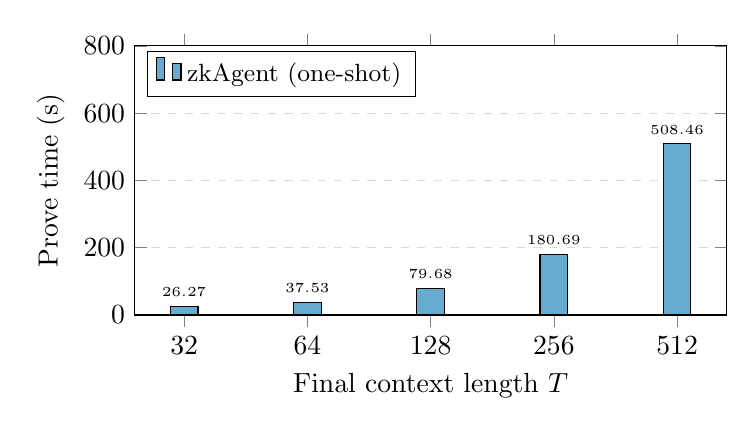
\begin{tikzpicture}
\begin{axis}[
  ybar, bar width=10pt,
  xlabel={Final context length $T$},
  ylabel={Prove time (s)},
  symbolic x coords={32, 64, 128, 256, 512},
  xtick=data,
  ymin=0, ymax=800,
  width=0.75\textwidth, height=5cm,
  legend style={at={(0.02,0.98)}, anchor=north west, font=\small},
  nodes near coords, every node near coord/.append style={font=\tiny},
  ymajorgrids=true, grid style={dashed, gray!30},
]
  \addplot[fill=positive!60] coordinates {(32,26.27) (64,37.53) (128,79.68) (256,180.69) (512,508.46)};
  \legend{zkAgent (one-shot)}
\end{axis}
\end{tikzpicture}
\end{center}

\vspace{-2pt}
\begin{tabular}{@{}lrrrrr@{}}
\toprule
& $T=32$ & $T=64$ & $T=128$ & $T=256$ & $T=512$ \\
\midrule
zkGPT prove (s) & 65.01 & 1,727.8 & 7,881.0 & 33,867.9 & \neg{149,192.6} \\
\textbf{Ours} prove (s) & 26.27 & 37.53 & 79.68 & 180.69 & \pos{508.46} \\
Speedup & 2.5$\times$ & 46$\times$ & 99$\times$ & 187$\times$ & \pos{294$\times$} \\
\bottomrule
\end{tabular}
\end{frame}

\begin{frame}{Evaluation: End-to-End Agent Performance}
\begin{columns}[T]
\column{0.55\textwidth}
Two realistic tool-using tasks on GPT-2:

\vspace{4pt}
\begin{tabular}{@{}lrr@{}}
\toprule
& \textbf{Weather} & \textbf{Coding} \\
\midrule
Transcript length & 154 tokens & 146 tokens \\
\midrule
Inference prove & 230.14\,s & 225.63\,s \\
Schema prove & 2.87\,s & 2.78\,s \\
Tool prove & 3.25\,s & 3.90\,s \\
\midrule
\textbf{Total prove} & \pos{236.26\,s} & \pos{232.31\,s} \\
\textbf{Verify} & \pos{0.37\,s} & \pos{0.49\,s} \\
\textbf{Proof size} & 42.55\,MB & 42.38\,MB \\
\bottomrule
\end{tabular}

\column{0.42\textwidth}
\textbf{Key observations}:
\begin{itemize}
  \item Inference proof dominates ($>97\%$)
  \item Schema + tool overhead is small ($\sim$3\%)
  \item Verification: sub-second
  \item Proof size: $\sim$42\,MB (practical for transmission)
\end{itemize}

\vspace{4pt}
\HL{First practical end-to-end verifiable agent execution.}
\end{columns}
\end{frame}

\begin{frame}{Scaling: Preprocessing and Larger Models}
\textbf{Embedding preprocessing} across representative models (one-time cost):

\vspace{4pt}
\begin{center}
\begin{tabular}{@{}llrrr@{}}
\toprule
Model & $(N, d)$ & Preproc.\ (s) & Size (GB) \\
\midrule
GPT-2 & $(50257, 768)$ & 759.9 & 4.52 \\
TinyLlama & $(32000, 2048)$ & 929.8 & 6.01 \\
GPT-2 XL & $(50257, 1600)$ & 1,536.3 & 9.40 \\
DeepSeek V2 & $(102400, 4096)$ & 8,264.4 & 48.05 \\
GPT-3 & $(50257, 12288)$ & 11,735.0 & 72.03 \\
DeepSeek V3 & $(129280, 7168)$ & 14,505.4 & 84.05 \\
\bottomrule
\end{tabular}
\end{center}

\vspace{4pt}
\textbf{RoPE optimization on Llama-2-7B}: $95.70$s $\to$ $3.06$s per layer $\Rightarrow$ \pos{$-2{,}964$s} across 32 layers.

\vspace{2pt}
\textbf{Shout for decoding}: \pos{10.7$\times$--24.4$\times$} faster than zkGPT's lookup backend.
\end{frame}

% ============================================================
% PART 7: CLOSING
% ============================================================

\begin{frame}{Conclusion and Open Problems}
\textbf{zkAgent}: first practical system for \pos{verifiable agent execution}.

\vspace{4pt}
\begin{columns}[T]
\column{0.48\textwidth}
\textbf{Three contributions}:
\begin{enumerate}
  \item \textbf{Complete inference proof}: embedding lookup (cq), RoPE (Hadamard), decoding (range checks)
  \item \textbf{One-shot transcript proving}: causal mask $\Rightarrow$ single forward pass proves entire agent run
  \item \textbf{Verifiable tool binding}: zkTLS + zkVM + Coral, composed with inference proof
\end{enumerate}

\column{0.48\textwidth}
\textbf{Open directions}:
\begin{itemize}
  \item Scale to \textbf{larger models} (7B+) --- prover time still dominated by Transformer
  \item \textbf{More tool types} (databases, multi-modal, human-in-the-loop)
  \item \textbf{Privacy-preserving} agents: hide model weights \emph{and} user queries
  \item \textbf{Proof size reduction}: Dory commitment $\Rightarrow$ $O(1)$ vs.\ $O(\sqrt{\ell n})$ with KZH
  \item \textbf{Hardware acceleration}: GPU/FPGA prover
\end{itemize}
\end{columns}
\end{frame}

\begin{frame}{References}
\begin{thebibliography}{9}
\small
\bibitem{zkgpt} D.\ Sun et al., ``zkGPT: Zero-Knowledge Proofs for Generative Pre-Trained Transformers,'' USENIX Security '25.
\bibitem{zkllm} Z.\ Sun et al., ``zkLLM: Zero Knowledge Proofs for Large Language Models,'' CCS '24.
\bibitem{zkml} B.-J.\ Chen et al., ``ZKML: An Optimizing System for ML Inference in Zero-Knowledge Proofs,'' EuroSys '24.
\bibitem{cq} L.\ Eagen, D.\ Fiore, A.\ Gabizon, ``cq: Cached Quotients for Fast Lookups,'' ePrint 2022.
\bibitem{shout} Lasso/Shout, ``Efficient lookup arguments via offline memory checking.''
\bibitem{coral} Brave Software, ``Coral: Bridging Parsing and Zero-Knowledge Proofs,'' IEEE S\&P '26.
\bibitem{gkr} S.\ Goldwasser, Y.\ T.\ Kalai, G.\ N.\ Rothblum, ``Delegating Computation: Interactive Proofs for Muggles,'' STOC '08.
\end{thebibliography}
\end{frame}

\begin{frame}
\centering
\vspace{2cm}
{\LARGE Thank You!}

\vspace{1cm}
{\large Questions?}
\end{frame}

% ============================================================
% BACKUP SLIDES
% ============================================================
\appendix
\begin{frame}{Backup Slides}
\centering
{\large Additional material for anticipated questions.}
\end{frame}

\begin{frame}{Backup: Prefix Equivalence (Proof Sketch)}
\label{slide:prefix-equiv}
\textbf{Claim}: under causal attention mask, the logits at position $i$ computed from the full transcript $\tr$ are identical to those computed from the prefix $\tr_{\leq i}$.

\vspace{6pt}
\textbf{Proof sketch}:
\begin{enumerate}
  \item Self-attention is the \textbf{only} cross-position sublayer. LayerNorm, MLP, residual connections are all position-wise.
  \item Causal mask enforces: for query position $i$, attention weights $\alpha_{ij} = 0$ for all $j > i$.
  \item Therefore, hidden state $\mathbf{h}_i^{(\ell)}$ at layer $\ell$ depends only on $\{\mathbf{h}_j^{(\ell-1)}\}_{j \leq i}$.
  \item By induction on layers: $\mathbf{h}_i^{(L)}$ (and hence $\boldsymbol{\ell}_i$) depends only on $\tr_{\leq i}$.
\end{enumerate}

\vspace{4pt}
This is standard in supervised fine-tuning (``teacher forcing''), but its application to \textbf{zero-knowledge proof batching} is novel.
\end{frame}

\begin{frame}{Backup: cq Lookup Argument}
\textbf{cq} (cached quotients) = logarithmic-derivative reduction + univariate KZG + preprocessing.

\vspace{4pt}
\textbf{Setup}: table $\mathbf{b} \in \F^N$ with interpolant $T(X)$ over domain $\mathcal{V}$:
\begin{itemize}
  \item Precompute Lagrange basis commitments $\{\mathrm{Com}(L_j)\}_{j \in [N]}$
  \item Precompute cached quotients $\{c_{Q,j}\}_{j \in [N]}$ where $L_j(X)T(X) = b_j L_j(X) + Z_\mathcal{V}(X)Q_j(X)$
\end{itemize}

\vspace{4pt}
\textbf{Online}: given query multiset $\{a_i\}_{i \in [\ell]}$, sample $\beta$ and prove:
\[
  (B(X) + \beta) \cdot F(X) - M(X) = Q(X) \cdot Z_\mathcal{H}(X)
\]
via pairing check. Sparsity: only combine basis/quotient terms for $\mathrm{supp}(\mathbf{m})$, so cost $\propto T$, not $N$.

\vspace{4pt}
\textbf{Our extension}: keep table side univariate (with preprocessing), query side multilinear (compatible with GKR).
\end{frame}

\begin{frame}{Backup: Quantization and Model Accuracy}
Following prior work, floating-point tensors $\to$ signed integers with public scale $s = c \cdot 2^e$.

\vspace{4pt}
\textbf{Perplexity evaluation} (GPT-2, WikiText-103):

\vspace{2pt}
\begin{center}
\begin{tabular}{@{}lccc@{}}
\toprule
Setting & FP32 baseline & Our quantization & Degradation \\
\midrule
GPT-2 (124M) & 29.16 & 29.44 & $< 1\%$ \\
\bottomrule
\end{tabular}
\end{center}

\vspace{4pt}
\textbf{End-to-end agent accuracy}: tested on weather-agent and coding-assistant tasks---quantized model produces identical tool calls and final answers as FP32 baseline on evaluated traces.

\vspace{4pt}
\textbf{Key insight}: modern LLMs are robust to moderate quantization; integer semantics preserve inference quality while enabling efficient finite-field arithmetization.
\end{frame}

\begin{frame}{Backup: Detailed Cost Comparison}
\textbf{Full comparison at $T = 512$, $T_0 = 30$ (GPT-2)}:

\vspace{4pt}
\begin{center}
\begin{tabular}{@{}lrrrr@{}}
\toprule
System & Prove (s) & Verify (s) & Proof size & Hardware \\
\midrule
ZKML & $>7{,}148$ (at $T\!=\!32$) & 17.61 & --- & CPU \\
zkLLM & $\sim 7{,}616$ (est.) & $\sim 260$ (est.) & --- & \textbf{GPU} (A100) \\
zkGPT & 149,192.6 & 4,361.09 & --- & CPU \\
\midrule
\textbf{zkAgent} & \pos{508.46} & \pos{0.51} & 108.23\,MB & CPU \\
\bottomrule
\end{tabular}
\end{center}

\vspace{4pt}
Notes:
\begin{itemize}
  \item zkLLM numbers estimated from per-step costs in zkGPT paper (run on GPU)
  \item Our comparison is \textbf{conservative}: zkAgent runs on CPU only
  \item Proof size dominated by Shout's sparse polynomial commitment ($O(\sqrt{\ell n})$ with KZH); switchable to Dory for $O(1)$
\end{itemize}
\end{frame}

\end{document}
